\section{Application to protoplanetary disks}\label{application} 
As a first application of our linear models, we estimate where in a
protoplanetary disk do the thermodynamic conditions allow the VSI to
operate. For a realistic disk one can consider the energy equation with
radiative cooling, 
%To connect our model with a realistic
%disk, we consider a more physically-motivated form of the energy
%equation with radiative cooling 
\begin{align}\label{real_energy}
%\rho T \frac{DS}{Dt} = - \left(\nabla\cdot\bm{F} - Q_+\right), 
\frac{\p P}{\p t} + \bm{v}\cdot\nabla P +\gamma P \nabla\cdot\bm{v} = - \frac{P}{\rho T
  c_v}\left(\nabla\cdot\bm{F} - Q_+\right), 
\end{align}where the temperature $T$ is defined through $P=\mathcal{R}\rho
T/\mu$, $\mathcal{R}$ is the ideal gas constant and $\mu$ is
the mean molecular weight, $c_v$ is the heat capacity at constant
volume, 
% In Eq. \ref{real_energy} $S$ is the
% specific entropy,
% \begin{align}
%   S \equiv c_v\ln{\left(\frac{p}{\rho^{\gamma}}\right)} 
% \end{align}
% where $c_v \equiv \left(\gamma-1\right)^{-1}\mathcal{R}/\mu$ is the
% specific heat capcity at constant volume
$\bm{F}$ is the radiative flux, and $Q_+$ is a heating
term such that an equilibrium solution exists. 

One should now model in detail each of the terms on the right
hand side (RHS) of Eq. \ref{real_energy}, linearize them, then solve
the resulting linear eigenvalue problem. Such an approach is beyond
the scope of this paper. Here, we simply model the RHS of
Eq. \ref{real_energy} such that it can be represented by a 
thermal relaxation time $t_c$ for the disk temperature. 
%Our aim is to relate the right hand side (RHS) of Eq. \ref{real_energy} to
%the 
To do so, we first consider separately perturbations
with radial lengthscales $l\equiv 2\pi/k_x\gg l_\mathrm{rad}$ and 
$l\ll l_\mathrm{rad}$, where      
\begin{align}\label{lrad}
  l_\mathrm{rad} \equiv \frac{1}{\kappa_d\rho} 
\end{align} 
is the photon mean-free-path and $\kappa_d$ is the (dust) opacity. 

%need to comment on kappa_d(rho,T) 

\subsection{Radiative diffusion}
Let us first consider perturbations with lengthscales $l\gg
l_\mathrm{rad}$. In this case, we assume  
temperature fluctuations are smoothed out by radiative diffusion. We
mode this in linear theory by writing the linearized RHS of
Eq. \ref{real_energy} as 
% we choose the heating term such that
% \begin{align}
%   Q_+ - \nabla\cdot\bm{F} \equiv \nabla\cdot\left[k_\mathrm{rad}\nabla
%     \left(T-T_{t=0}\right)\right], 
% \end{align} 
% where $k_\mathrm{rad}$ is the conduction coefficient to be defined
% implicitly. Eq. \ref{real_energy} becomes
% \begin{align}
%   \frac{DP}{Dt} = -\gamma P \nabla\cdot\bm{v} + \frac{P}{\rho T
%     c_v}\nabla\cdot\left[k_\mathrm{rad}\nabla\left(T-T_{t=0}\right)\right].     
% \end{align}
% When linearized, the last term on the RHS becomes
\begin{align}\label{diff_cool_proper}
  \frac{P}{\rho T c_v} \nabla\cdot\left(k_\mathrm{rad}\nabla\delta
    T\right),  
\end{align}
where $k_\mathrm{rad}$ is the conduction coefficient to be defined
implicitly.

However, Eq. \ref{diff_cool_proper} fundamentally changes the linear problem by
introducing higher order derivatives. We defer a proper analysis of
this problem to a follow-up study. Here, we are interested in
order-of-magnitude estimates for perturbations with radial
lengthscales much smaller than vertical lengthscales. We thus proceed
by assuming vertical derivatives can be neglected in
Eq. \ref{diff_cool_proper} and write  
\begin{align}\label{diff_cool_approx}
  \frac{P}{\rho T c_v} \nabla\cdot\left(k_\mathrm{rad}\nabla\delta
    T\right) &\to -\frac{k_\mathrm{rad}}{\rho
    c_v}k_x^2P\left(\frac{\delta T}{T}\right)\notag\\
  &\equiv -\eta k_x^2 \left(\delta P - \frac{P}{\rho}\delta\rho\right), 
\end{align}
% we are interested in radially-thin perturbations  
where $\eta=k_\mathrm{rad}/\rho c_v$ is the diffusion coefficient and
is given in terms of physical disk parameters as 
\begin{align}\label{eta_def}
  \eta = \frac{16\sigma_s T^3}{3\kappa_d\rho^2 c_v}, 
\end{align}
where $\sigma_s$ is the Stefan-Boltzmann constant. 
From Eq. \ref{diff_cool_approx} we identify the scale-dependent thermal relaxation
time for diffusion as 
\begin{align}\label{tc_diff_cool} 
  t_\mathrm{diff} = \frac{1}{\eta k_x^2}\equiv \frac{\Omega_k^{-1}}{\hat{\eta}\khat^2}, 
\end{align}
where $\hat{\eta} = \eta/H^2\Omega_k$ is the 
dimensionless diffusion coefficient. 


\subsection{Newtonian cooling}\label{newton_cool}
For perturbations with small lengthscales, $l\ll l_\mathrm{rad}$, 
the disk is optically thin. In this case, we assume 
Newtonian cooling can be applied, which is the thermal
relaxation model as adopted in our linear models. That is, temperature
flucations $\delta T$ decay on a timescale $t_\mathrm{cool}$,
independent of $k_x$. For simplicity, we take  
% the radiative cooling is given by {\bf (reference?)}
% \begin{align}
% \nabla\cdot\bm{F} = 4 \rho \kappa_d \sigma_s T^4,
% \end{align}   
% where $\sigma_s$ is the Stefan-Boltzmann constant. We choose the
% heating term 
% \begin{align}
%   Q_+ = 4\rho\kappa_d\sigma_s T^{4}_{t=0}. 
% \end{align}
% Then Eq. \ref{real_energy} becomes
% \begin{align}
%   \frac{DP}{Dt} = -\gamma P \nabla\cdot\bm{v} -
%   \frac{4P\kappa_d\sigma_s}{Tc_v}\left(T^4 - T_{t=0}^4\right), 
% \end{align}
% where $c_v$ is the heat capacity at constant volume. When linearized, the last term on the RHS becomes
% \begin{align}
%   -\frac{16\sigma_s}{c_v}\kappa_d T^3\left(\delta P -
%     \frac{P}{\rho}\delta\rho\right). 
% \end{align}
% By comparing this expression with the linearized version of the energy
% equation used in our calculations (Eq. \ref{full_energy1}), we identify 
% \begin{align}\label{tc_newton_cool} 
%   t_\mathrm{cool} = \frac{c_v}{16\sigma_s\kappa_dT^3}
% \end{align}
% as the thermal relaxation timescale for optically thin cooling. 
\begin{align}
t_\mathrm{cool} = \frac{l_\mathrm{rad}^2}{3\eta}. 
\end{align}

\subsection{A model for combined thermal relaxation}\label{toy_relax}
To unify $t_\mathrm{cool}$ and $t_\mathrm{diff}$, we define the
effective thermal relaxation timescale in linear theory as
\begin{align}\label{tc_def}
  t_c &\equiv t_\mathrm{cool} + t _\mathrm{diff}. %=
 % \frac{l_\mathrm{rad}^2}{3\eta} + \frac{1}{\eta k_x^2},  
\end{align}
%where the relation between $t_\mathrm{cool}$, $l_\mathrm{rad}$ and
%$\eta$ can be inferred from Eq. \ref{lrad}, Eq. \ref{tc_newton_cool}
%and Eq. \ref{eta_def}. 
Eq. \ref{tc_def} is a simple prescription so
that for small scales (large $k_x$), $t_c\to t_\mathrm{cool}$, while
for large scales (small $k_x$), $t_c\to t_\mathrm{diff}$. Writing the
volume density $\rho = \Sigma\hat{\rho}/\sqrt{2\pi}H$, where
$\hat{\rho} = \rho/\rho_0$ and $\Sigma$ is the surface density at the
radius of interest, the 
% In order to utilize our linear results, which assumes $t_c$ is a
% constant, we need to make further 
% approximations. Specifically, we consider vertically-isothermal disks
% and replace explicit $\rho$ dependencies in the above expressions by $\Sigma/
% H$, where $\Sigma$ is the surface density at the fiducial
% radius of interest. For example, the dimensionless diffusion
% coefficient becomes 
% \begin{align}\label{diff_coeff_dimensionless}
%   \hat{\eta} \to  \frac{16\sigma_s T^3}{3\kappa_d\Sigma^2
%     c_v\Omega_k}. 
% \end{align}
% Furthermore, we will choose a temperature-dependent opacity model for
% simplicity, so that $\kappa_d=\kappa_d(T)$.
dimensionless thermal
relaxation time $\beta$ becomes 
\begin{align}\label{real_beta}
  \beta(z;\khat) \equiv t_c\Omega_k =
  % \frac{1}{\hat{\eta}}\left[\frac{l_\mathrm{rad}^2}{3H^2}
  %   + \frac{\hat{\rho}^2(z)}{2\pi\khat^2}\right]  \simeq
  \frac{1}{\hat{\eta}}\left[\frac{1}{3\kappa_d^2\Sigma^2} 
    + \frac{\hat{\rho}^2(z)}{2\pi \khat^2}\right].
\end{align}
Note that the thermal relaxation time depends on both the perturbation lengthscale $\khat$ 
and distance from the midplane. %The latter is due to the density-dependence in the diffusion time. 
%is then a constant for vertically-isothermal disks, 
%and we can directly apply previous results. 

\subsection{Evaluation for a fiducial disk model}
We evaluate Eq. \ref{real_beta} for the protoplanetary disk model
described in \cite{chiang10} and summarized in Appendix \ref{mmsn}
(where an opacity model is also chosen). Defining $r_\mathrm{AU}\equiv
r/\mathrm{AU}$, we find Eq. \ref{real_beta} becomes
\begin{align}\label{beta_mmsn}
  \beta(z; \khat) =
  &\frac{4.4\times10^5}{\mu(\gamma-1)}\left(\frac{\hat{\kappa}_d\hat{\Sigma}^2}{\hat{T}}\right)r_\mathrm{AU}^{-57/14}\notag\\
&\times\left[\frac{8.3\times10^{-9}}{\hat{\kappa}_d^2\hat{T}^4\hat{\Sigma}^2}r_\mathrm{AU}^{33/7}+\frac{\hat{\rho}^2(z)}{2\pi\khat^2}\right].     
\end{align}
We refer to the case with the scalings
$\hat{\Sigma}=\hat{\kappa}_d=\hat{T}=1$ as the Minimum Mass Solar
Nebulae (MMSN). The physical thermal relaxation timescale
$\beta$ is height-dependent, whilst for analytical discussion we
assumed it is constant. Nevertheless, it is instructive to evaluate
and compare with the criterion Eq. \ref{iso_vsi_cond} for the fiducial  
disk model,  
\begin{align}\label{bcrit_mmsn}
  \beta_\mathrm{crit} = \frac{1.44\times10^{-2}}{(\gamma
    -1)}\left(\frac{\hat{T}}{\mu}\right)^{1/2}r_\mathrm{AU}^{2/7}. 
\end{align}
We recall $\beta < \beta_\mathrm{crit}$ is necessary for the
fundamental VSI when $\khat\gg 1$. %For $\khat\to0$, this
%becomes a sufficient condition (see Fig. \ref{relax_bcrit} and
%\S\ref{iso_vsi_beta_crit}). 

In Fig. \ref{mmsn_bcrit_bcool} we plot Eq. \ref{beta_mmsn}  with $\mu
=2.33$ and $\gamma=1.4$.  We set the scaling $\hat{T}=\hat{\Sigma}=1$
and consider three opacity scales: $\hat{\kappa}_d=0.1, \,1 $ and $10$
at two heights: $z=0$ and $z=3H$. We also plot Eq. \ref{bcrit_mmsn} in
each panel for comparison. 

Consider first the MMSN shown in the middle panels of
Fig. \ref{mmsn_bcrit_bcool}. The critical thermal timescale,
Eq. \ref{bcrit_mmsn}, as derived from our analytical discussion, is
most useful to assess the VSI in the optically thin regime (where the
curves overlap), since in this limit $\beta$ does not depend on
height. We can therefore conclude that the VSI can operate at tens of
AU in the MMSN. 

In the inner few AU of the MMSN, however, $\beta$  has a
strong dependence on height because the disk is optically thick. Given
a fixed $\khat$, one can have $\beta > \beta_\mathrm{crit}$ at the
midplane, but eventually $\beta<\beta_\mathrm{crit}$ with increasing
height. Our analytical criteria is not valid for variable $\beta$, but
given that the VSI depends on vertical shear, an effect that becomes
important away from the disk midplane, the inner disk may still be
able to develop the VSI, but it is likely restricted to the disk
surface.   

Now consider lowering the opacity, as shown in the top panels of
Fig. \ref{mmsn_bcrit_bcool}. The curves shift inward, but raises also
them. In fact, lowering the opacity by an order of magnitude renders
$\beta > \beta_\mathrm{crit}$ even away from the midplane. This
suggests that fiducial  disk stable to the fundametal mode for the
range of wavenumbers considered.  

Raising the opacity, as shown in the lower panels of
Fig. \ref{mmsn_bcrit_bcool}, decreases the thermal timescales, but
also shifts the curves outward, so the fundamental mode is restricted
to larger radii.  

%We remark that it is possible to satisfy $\beta<\beta_\mathrm{crit}$
%at small radii by choosing a sufficiently large $\khat$. However, our
%linear calculations suggest growth rates eventually decay as 
%$\khat\to\infty$. Thus, very small-scale VSI in the inner disk is
%probably unimportant.   

\begin{figure*}
  \includegraphics[scale=.47,clip=true,trim=0cm 1.8cm 0cm
  0cm]{figures/bcrit_mmsn_kap0d1_z0}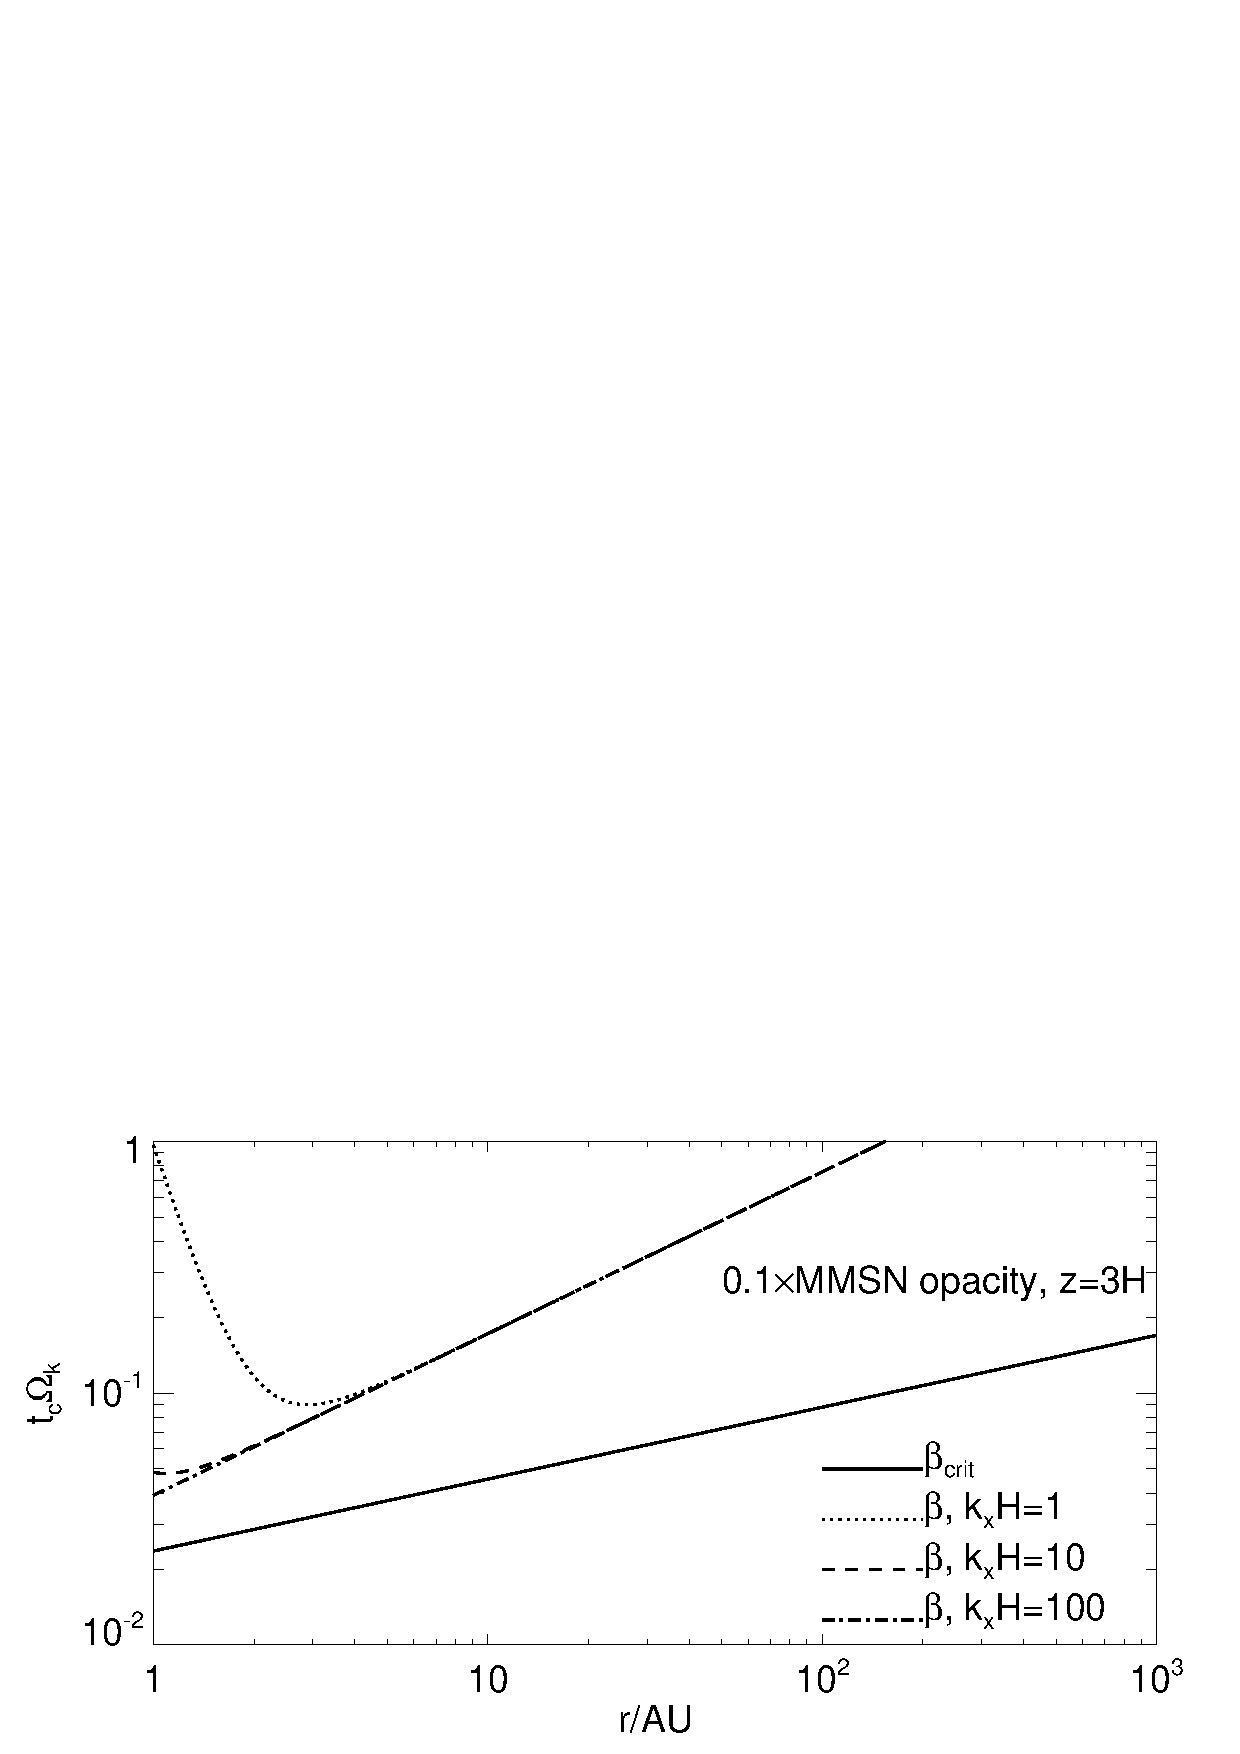
\includegraphics[scale=.47,clip=true,trim=2.5cm 1.8cm 0cm
  0cm]{figures/bcrit_mmsn_kap0d1_z3}\\ 
  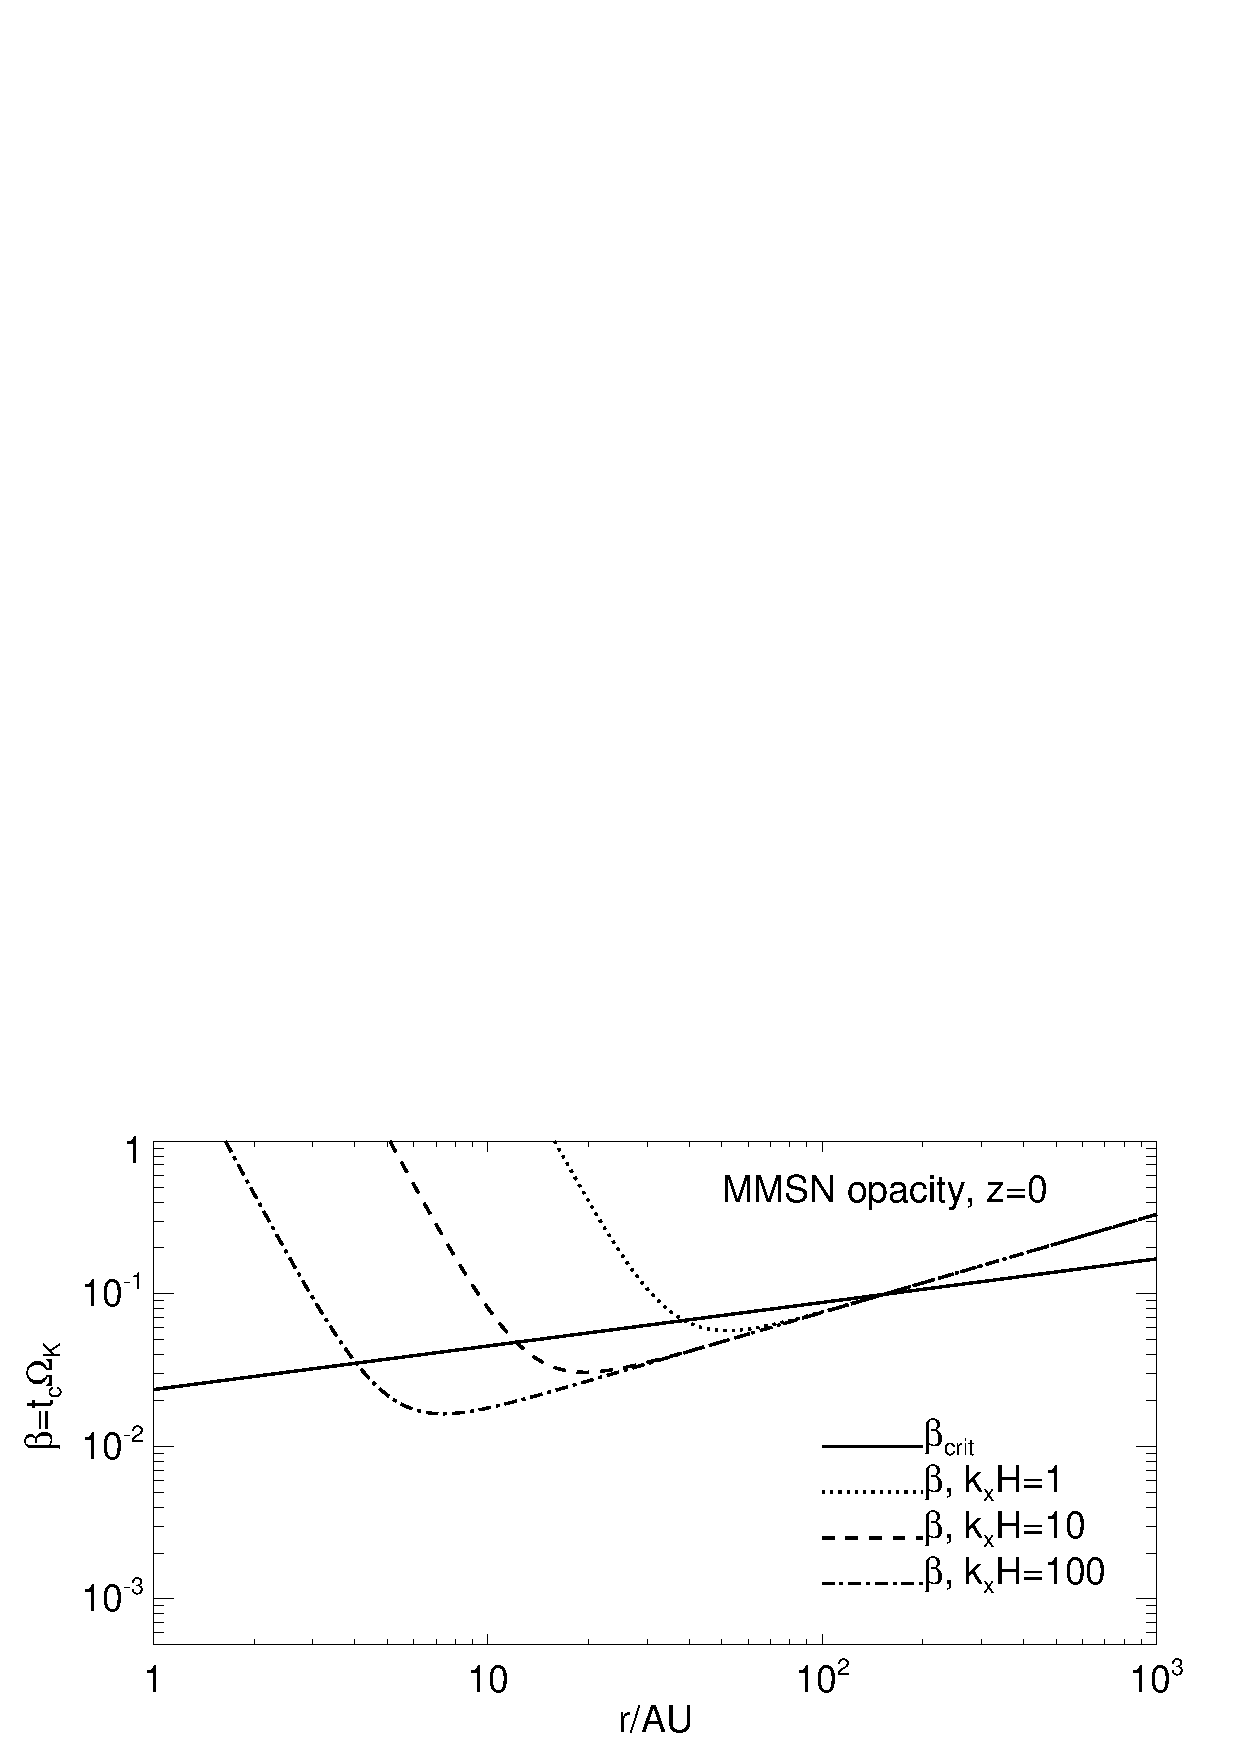
\includegraphics[scale=.47,clip=true,trim=0cm 1.8cm 0cm
  1cm]{figures/bcrit_mmsn_kap1_z0}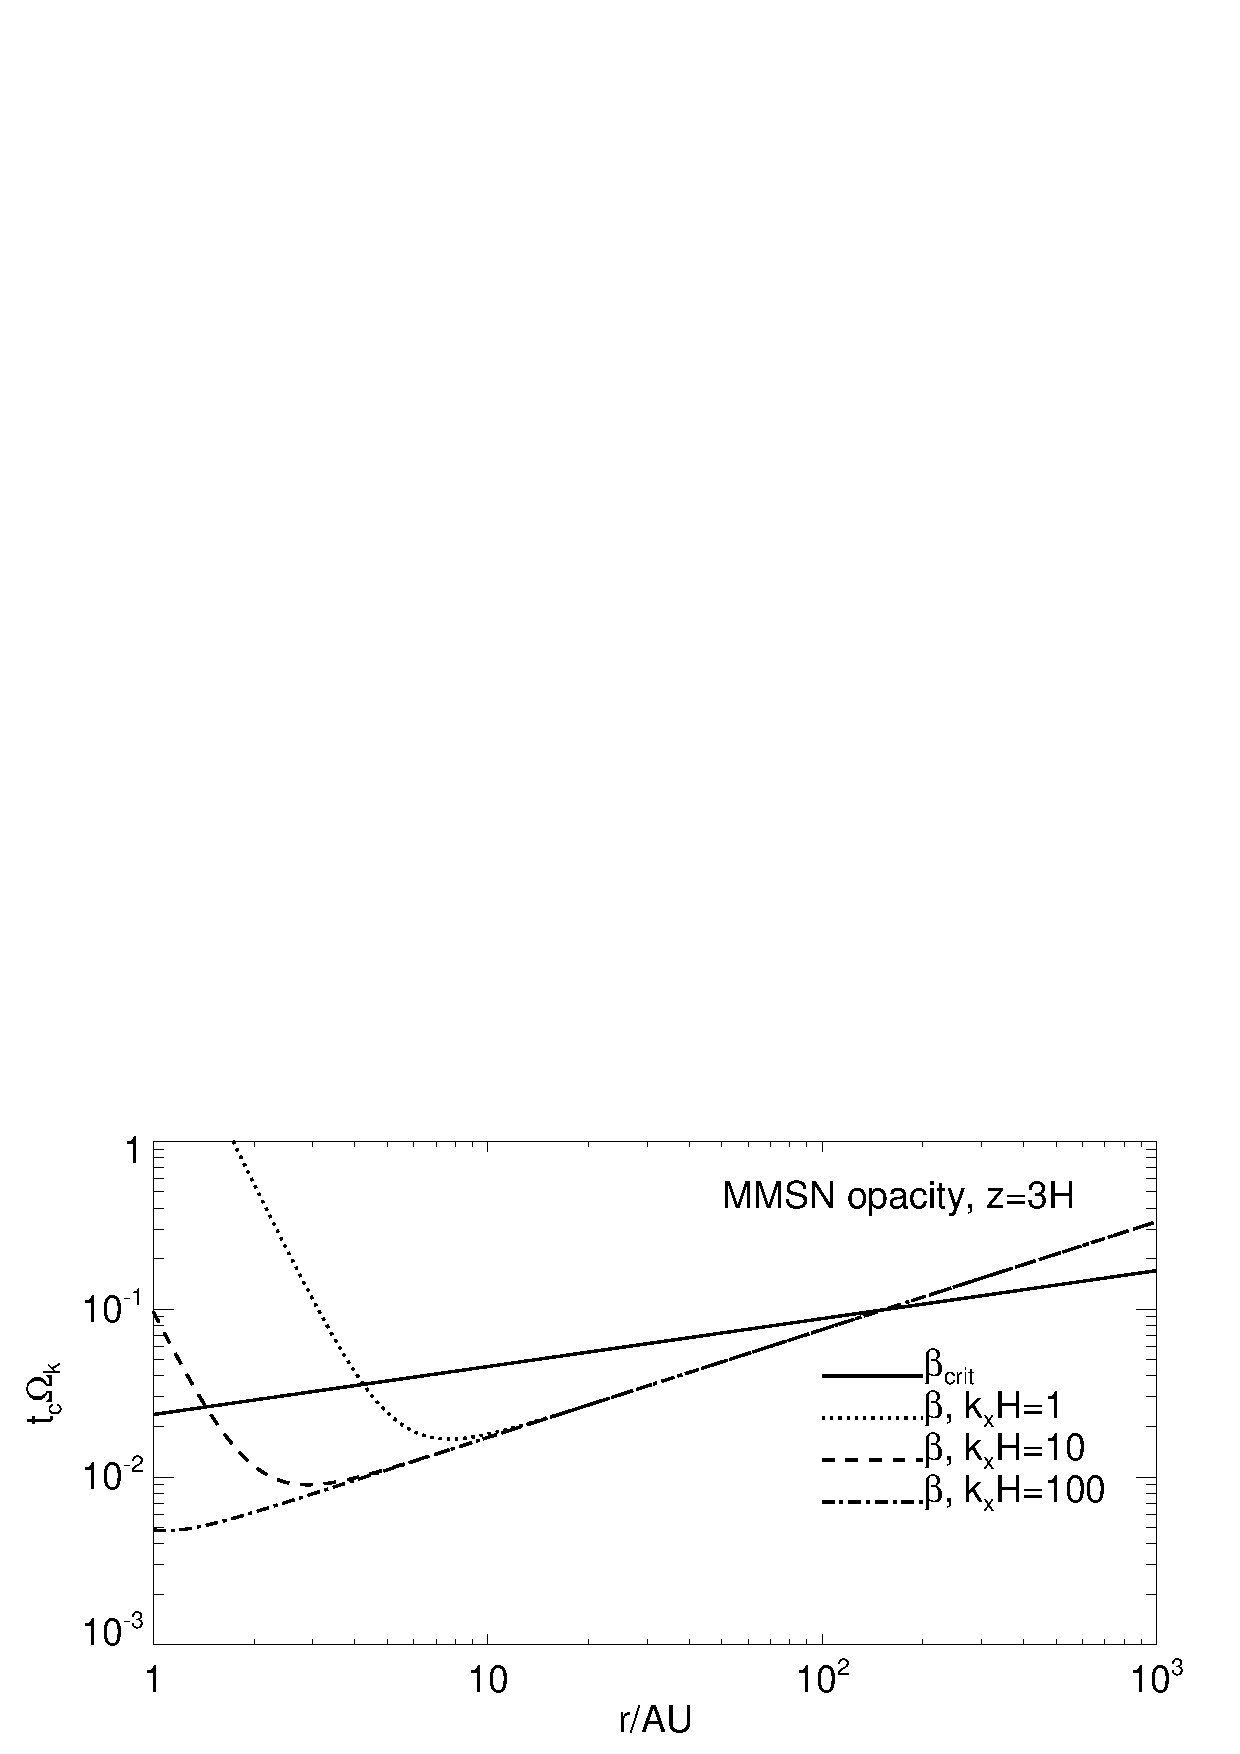
\includegraphics[scale=.47,clip=true,trim=2.5cm
  1.8cm 0cm 1cm]{figures/bcrit_mmsn_kap1_z3}\\
  \includegraphics[scale=.47,clip=true,trim=0cm 0cm 0cm
  1cm]{figures/bcrit_mmsn_kap10_z0}\includegraphics[scale=.47,clip=true,trim=2.5cm 0cm 0cm
  1cm]{figures/bcrit_mmsn_kap10_z3} 
  \caption{Dimensionless thermal relaxation timescales $\beta$,
    evaluated at the midplane (left) and at $z=3H$ (right) in the
    fiducial protoplanetary disk. Eq. \ref{beta_mmsn} is plotted  
    for three values of the 
    perturbation radial wavenumber: $\khat=1$ (dotted), $\khat=10$
    (dashed) and $\khat=100$ (dashed-dot), for three values of the
    opacity relative to the MMSN: $\hat{\kappa}_d=0.1$ (top),
    $\hat{\kappa}_d=1$ (middle) and $\hat{\kappa}_d=10$ (bottom).  
    The solid line is the 
    critical thermal relaxation timescale $\beta_\mathrm{crit}$. 
    % and 
    % $\beta<\beta_\mathrm{crit}$ is necessary for the fundamental isothermal VSI to operate  
    % for $\khat\gg1$. 
    \label{mmsn_bcrit_bcool}}   
\end{figure*}  

We remark that it is possible to satisfy $\beta <
\beta_\mathrm{crit}$ by choosing a sufficiently large $\khat$, or 
equivalently a sufficiently small perturbation lengthscale. We
illustrate this by plotting at each radius the value of $\khat$ such
that $\beta = \beta_\mathrm{crit}$. In the inner few AU of the MMSN,
one needs to consider large values of $\khat$ and/or regions away from
the disk midplane. 

% However, our linear
% calculations indicate growth rates eventually decay as one increases
% $\khat$. This, together with our finding of high $\khat$ modes may be
% affected by vertical boundary conditions, suggest the VSI does not
% operate in the inner few AU in protoplanetary disks where thermal
% relaxation is entirely due to radiation \citep[cf.][]{stoll14}.


\begin{figure}
  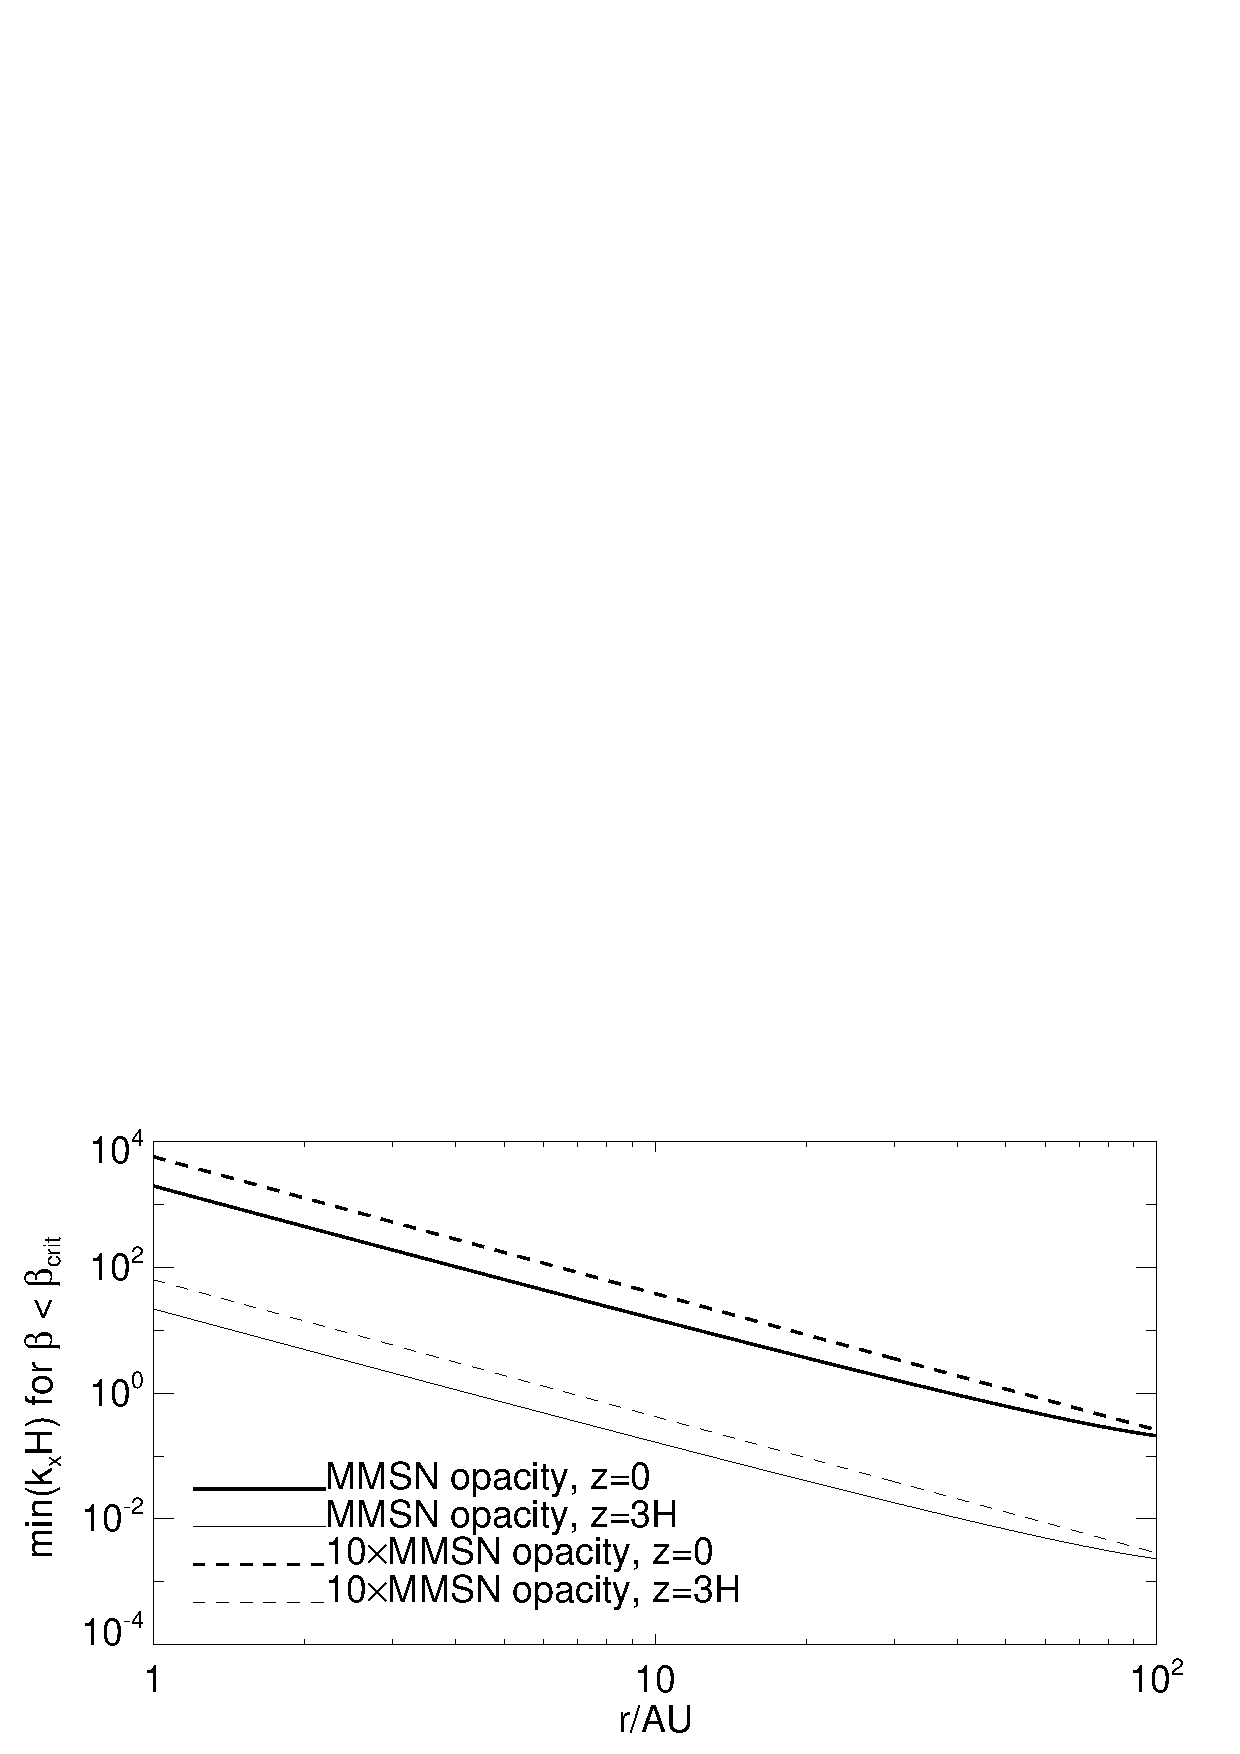
\includegraphics[width=\linewidth]{figures/bcrit_mink} 
  \caption{The minimum perturbation wavenumber $\khat$ in
    the MMSN such that the associated dimensionless thermal
    relaxation time  $\beta$ at $z=0$ (thick lines) and $z=3H$ (thin
    lines) is less than the critical timescale $\beta_\mathrm{crit}$.  
    \label{mmsn_bcrit_bcool_mink}}   
\end{figure}  


\subsection{Numerical examples}\label{mmsn_example}
Here we solve the linear stability problem with the
thermal relaxation function defined by Eq. \ref{beta_mmsn}. We
consider the MMSN at $r=50$AU and $r=2$AU. 

We first compare $\beta$ at these radii in Fig. \ref{beta_compare}. In
the optically thin outer disk, $\beta$ is independent of $z$ and
$\beta<\beta_\mathrm{crit}$ throughout the disk column. We thus expect
the VSI to operate at $r=50$AU. In the inner disk, $\beta$ depends on 
height such that $\beta\lesssim\beta_\mathrm{crit}$ only for 
$|z|\gtrsim 2H$, which suggest that the VSI will be restricted
restricted to the upper and lower layers in the inner disk.   

\begin{figure}
  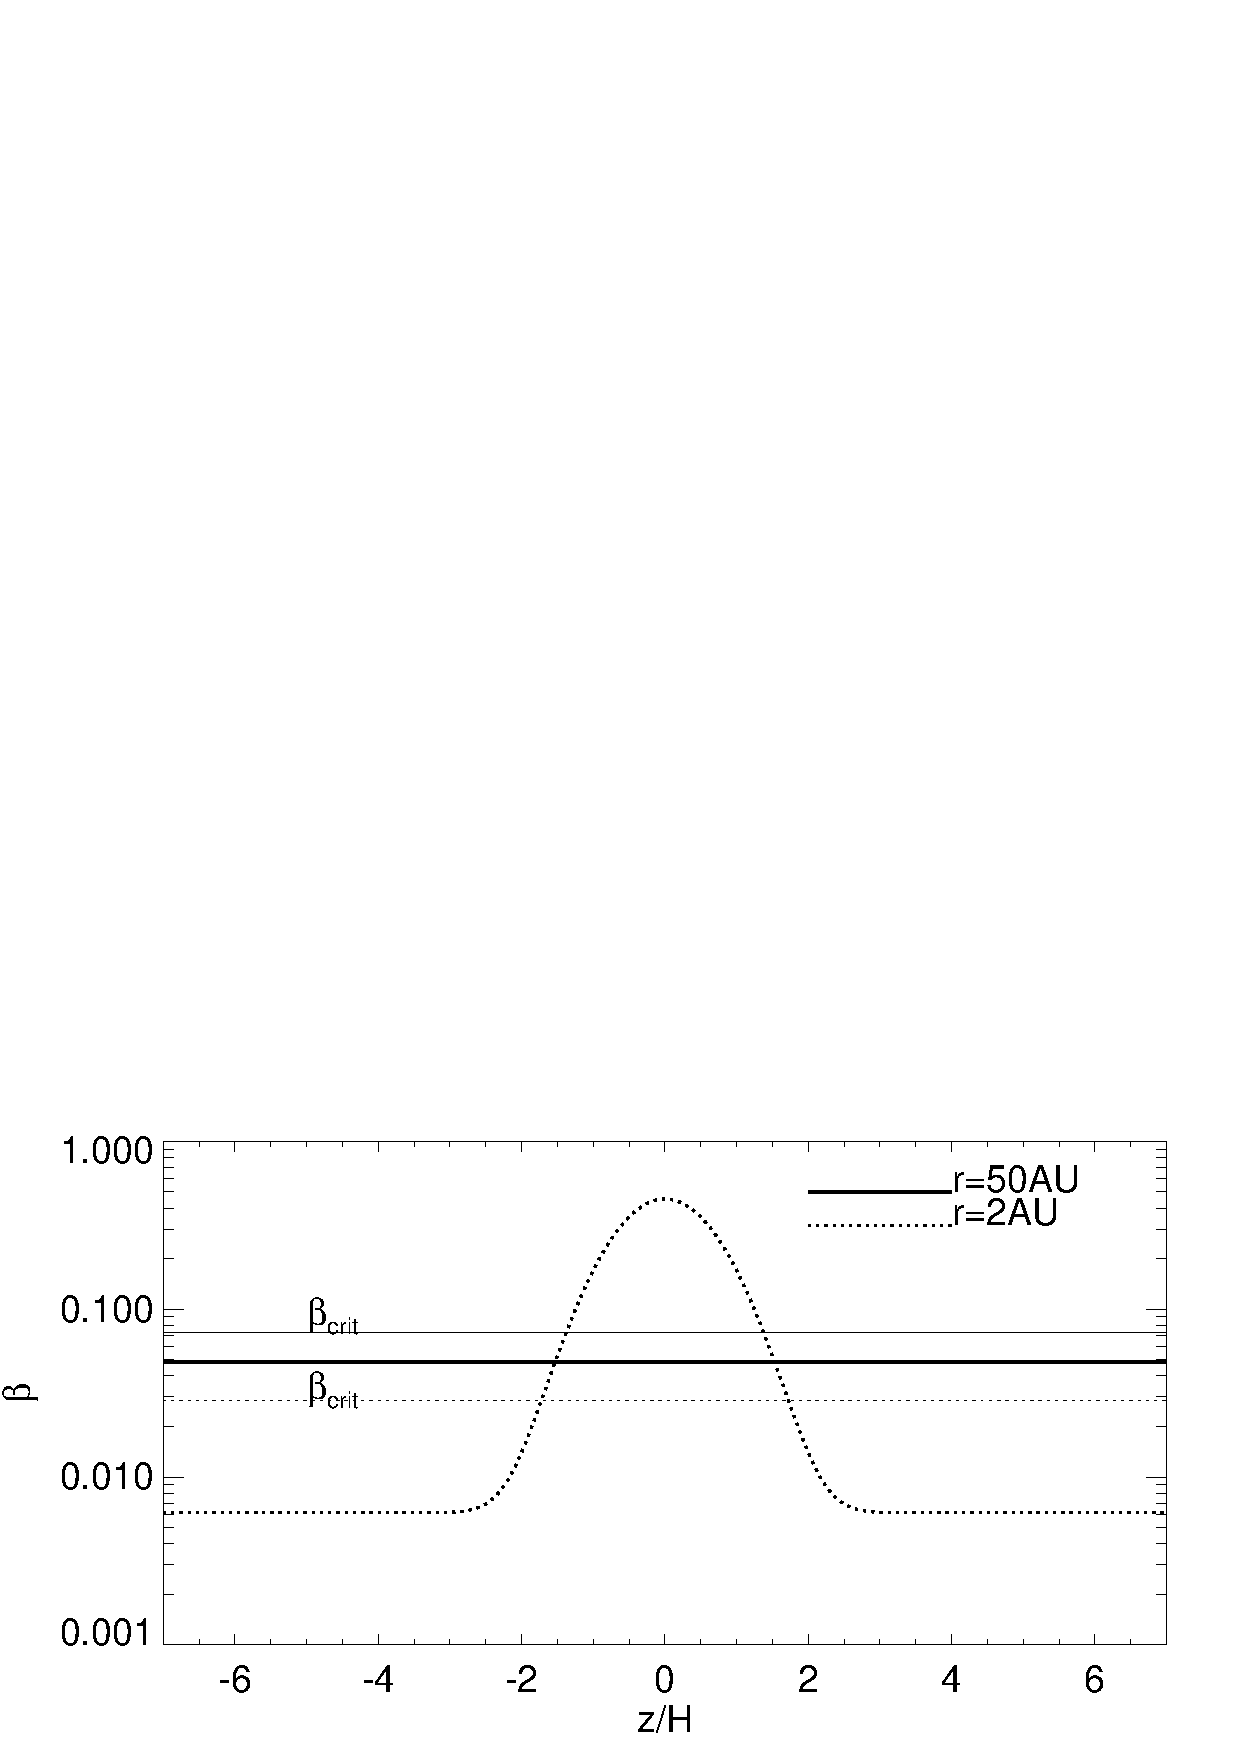
\includegraphics[width=\linewidth,clip=true,trim=0cm 0cm 0cm
  0cm]{figures/beta_compare} 
  \caption{Thermal relaxation timescales in the MMSN at $r=50$AU
    (thick solid) and $r=2$AU (thick dotted) for perturbation
    wavenumbers $\khat=10,\,100$, respectively. The corresponding
    horizontal lines are the critical thermal relaxation timescales
    derived in linear theory. 
    \label{beta_compare}}  
\end{figure}

In Fig. \ref{eigen_compare_mmsn} we compute growth rates of the
fundamental mode at $r=50$AU and $r=2$AU. At $r=50$AU growth rates are
insensitive to $\khat$ for $1\lesssim \khat\lesssim 60$, and
corresponds to growth time $\simeq 40$ local orbits. In the inner disk
at $r=2$AU, we only found unstable modes for $\khat\gtrsim50$. To
obtain a similar growth timescale at $r=2$AU requires $\khat\sim
100$. This is consistent with the expectation that, as we proceed into
the inner disk, it bcomes optically thick, so one needs to consider
smaller perturbation wavelengths to obtain a sufficiently short
thermal timescale.  

% In both cases we find that increasing $\khat$ increases the
% perturbation amplitudes near the disk surface. Such modes may be
% affected by boundary conditions so their robustness is unclear. 

\begin{figure}
  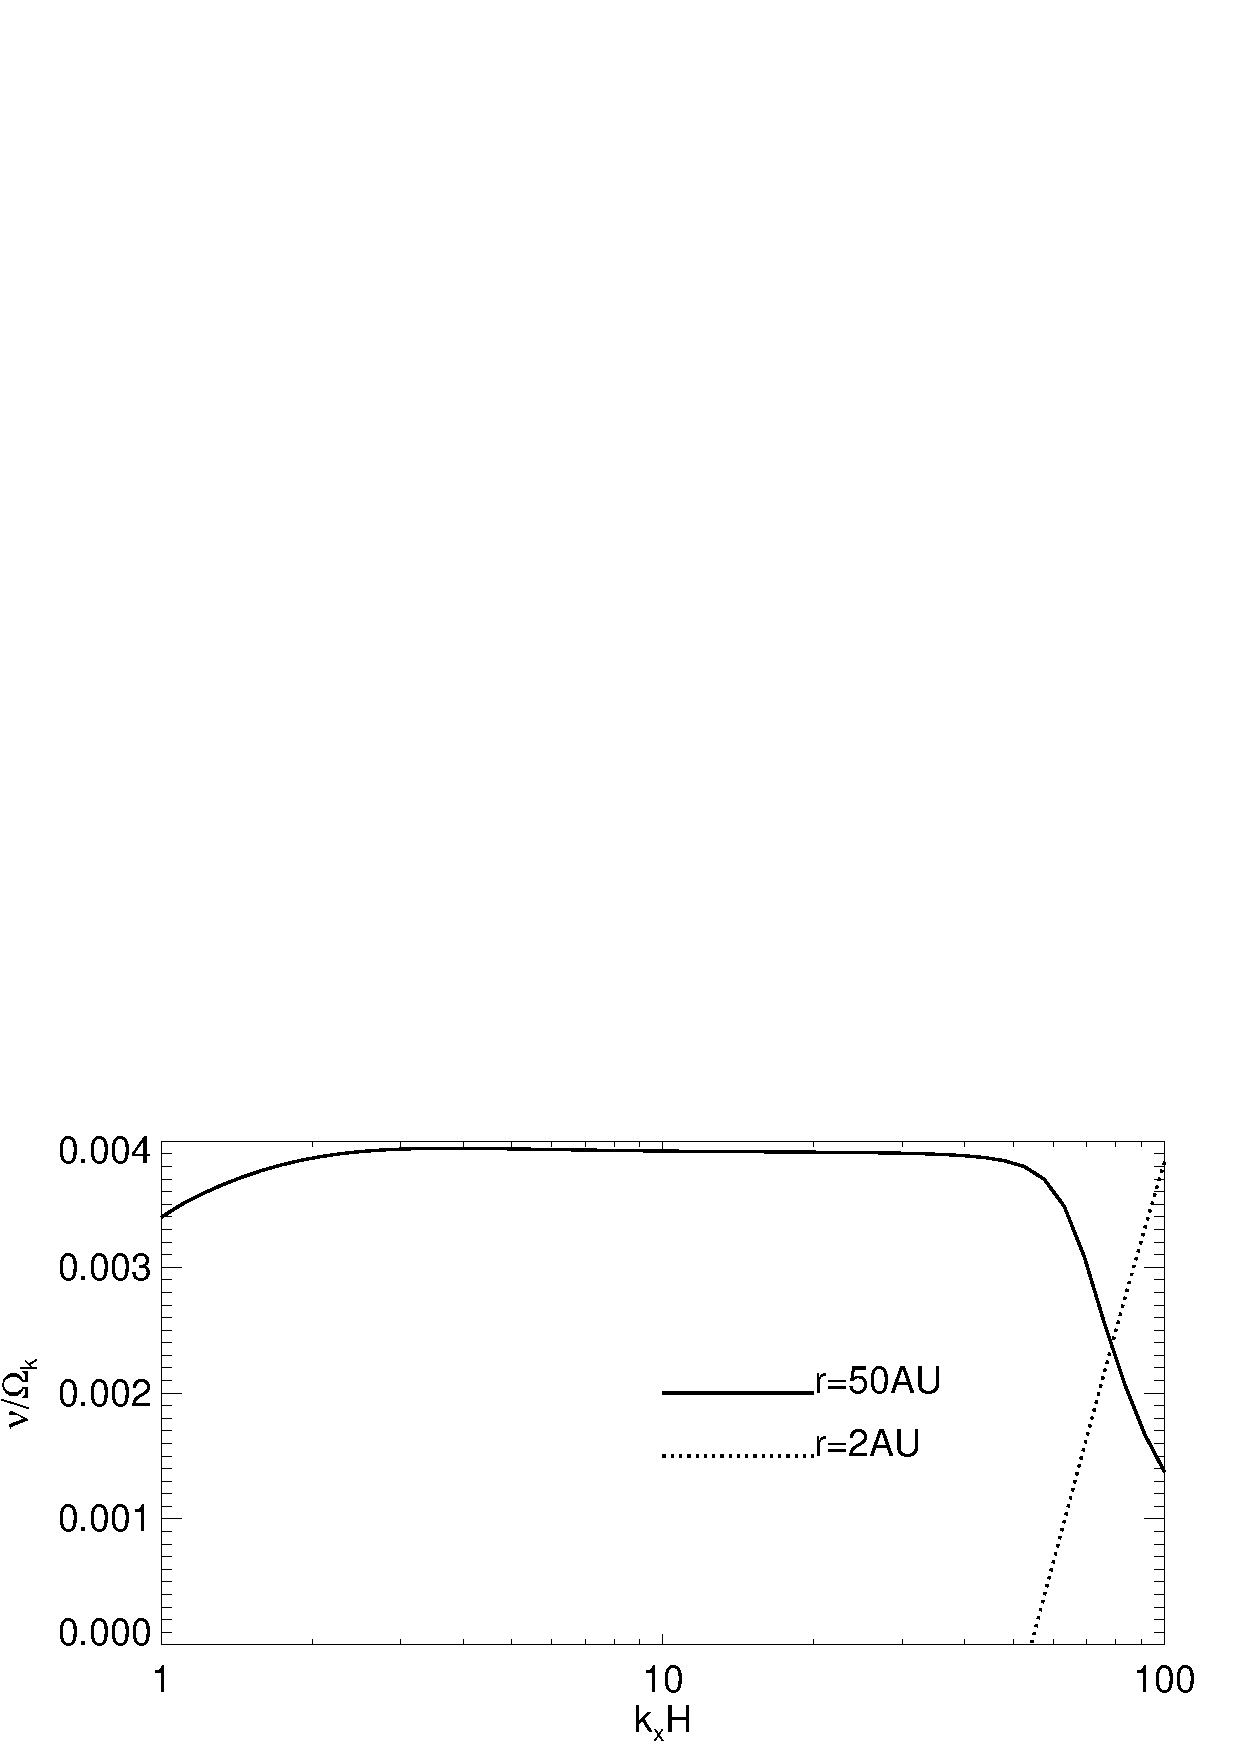
\includegraphics[width=\linewidth,clip=true,trim=0cm 0cm 0cm
  0cm]{figures/eigen_compare_grow_mmsn} 
  \caption{Growth rates of the fundamental VSI mode in the MMSN at
    $r=50$AU (solid) and $r=2$AU (dotted). 
    \label{eigen_compare_mmsn}}  
\end{figure}

Finally, we compare eigenfunctions for the vertical velocity at these
radii in Fig. \ref{mmsn_eigenvz}. We compare cases with similar growth
rates. At $r=50$AU we have vertical motion throughout the disk column
because the thermal timescale is less than critical. By contrast, at
$r=2$AU there is little vertical motion in $|z|\lesssim 2H$. 
Considering this result with Fig. \ref{beta_compare} suggests, but does
not prove, that the critical thermal timescale gives an indication of
where the VSI operates even when $\beta$ depends on $z$.  

%can always go to sufficiently large heights to get beta < beta crit,
%but getting close to boundaries/lower densities 

\begin{figure}
  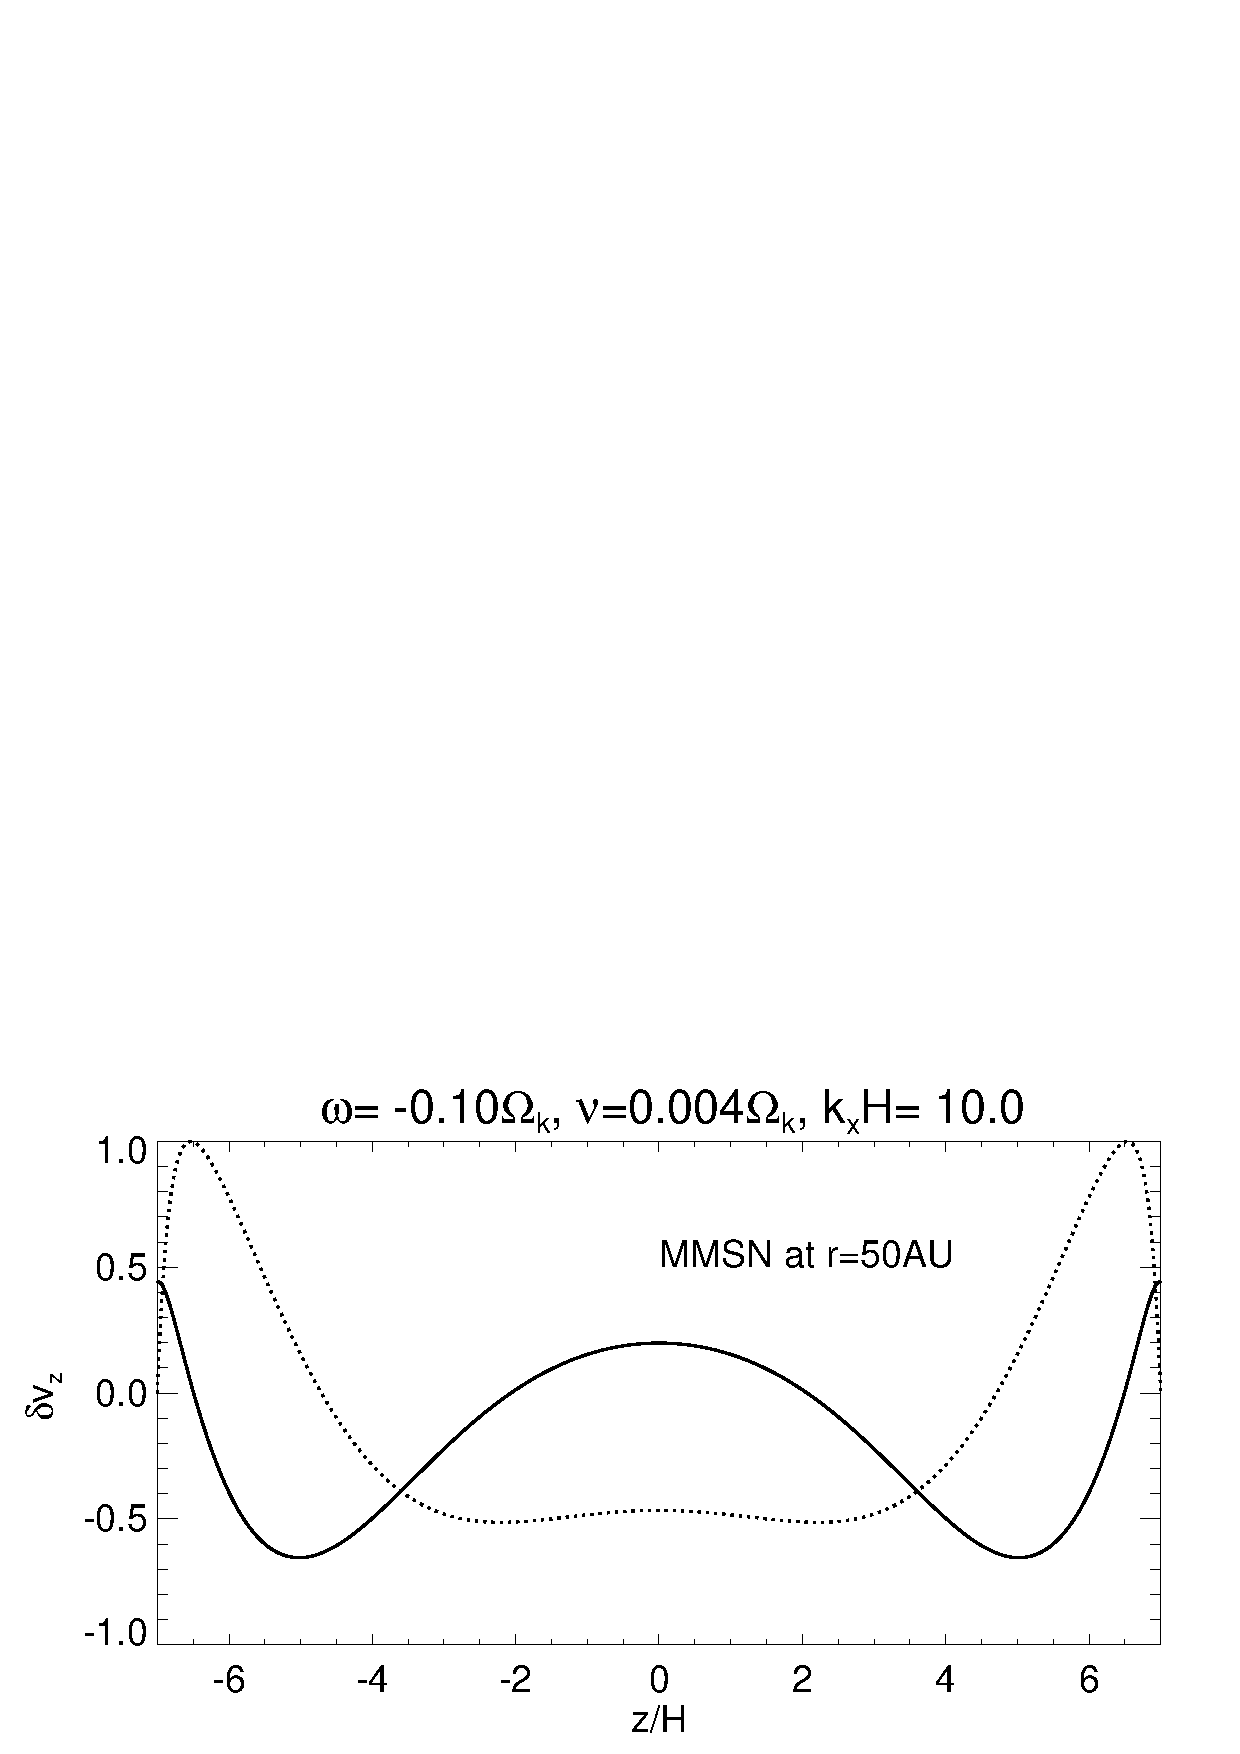
\includegraphics[width=\linewidth,clip=true,trim=0cm 1.75cm 0cm
  0cm]{figures/eigenvectorvz_mmsn_50AU}
  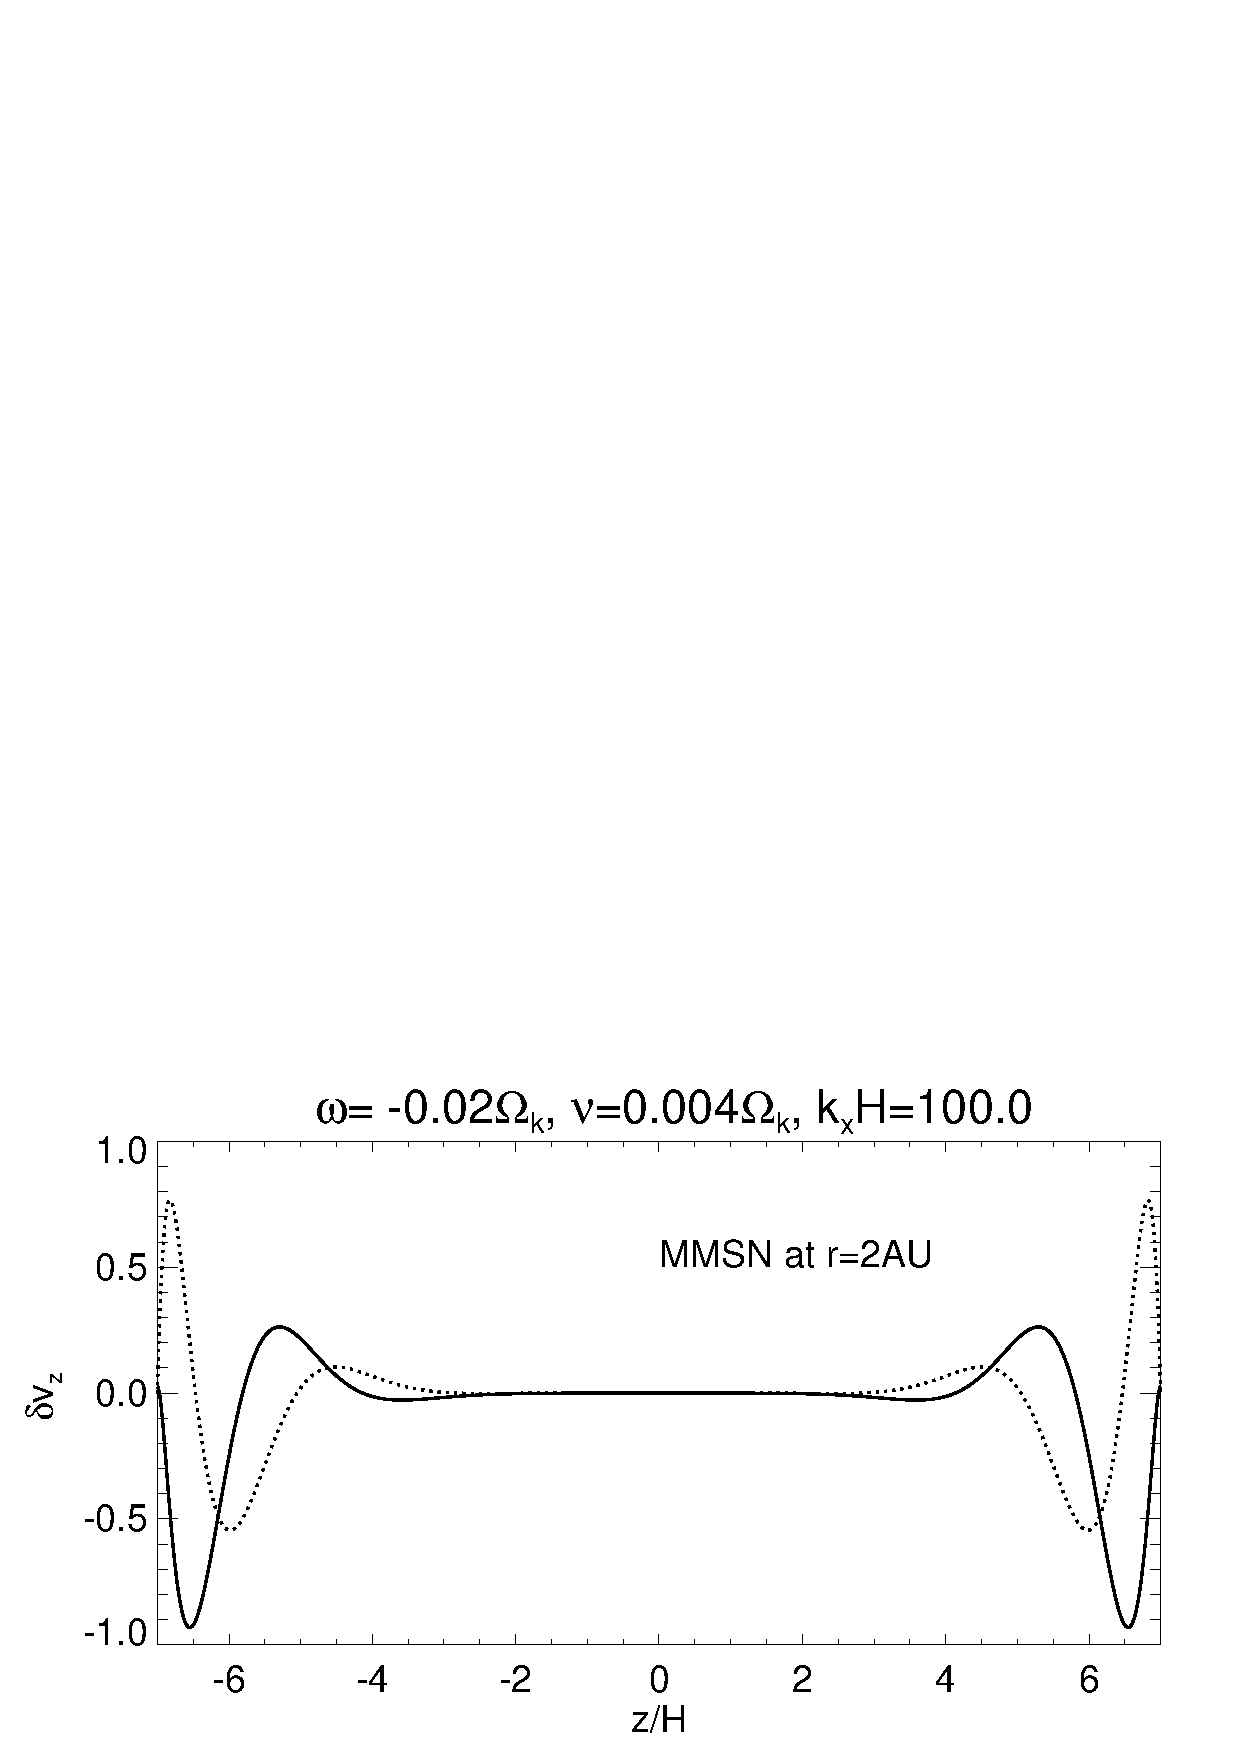
\includegraphics[width=\linewidth,clip=true,trim=0cm 0.0cm 0cm
  0cm]{figures/eigenvectorvz_mmsn_2AU}
  \caption{Comparison of vertical velocity perturbations of 
    fundamental VSI modes of similar growth rates in the MMSN at
    $r=50$AU (top) and $r=2$AU (bottom). The real (imaginary) part of
    $\delta v_z$ is shown as 
    the solid (dotted) curves. The eigenfunction has been normalized
    such that $\imag(\delta v_z)=0$ at the vertical boundaries, and
    $\mathrm{max}|\delta v_z|=1$. \label{mmsn_eigenvz}}      
\end{figure}
% only find one unstable mode -> close to marginal 
% larger kx 










\subsection{VSI in the outer parts of the MMSN}
To obtain an overall picture of the relevance of the VSI to the MMSN,
we calculate characteristic growth times $t_\mathrm{grow} = 1/\nu$ of 
the fundamental mode in units of the local Keplerian orbital period
$P_\mathrm{orb}= 2\pi/\Omega_k$. The results are shown in 
Fig. \ref{mmsn_overall} for perturbation wavenumbers $5\lesssim
\khat\lesssim 50$. We consider this range because for  
$\khat=O(1)$ or $\khat=O(10^2)$ we found eigenfunctions have large
amplitudes near the vertical boundaries, so such modes may be affected
by boundary conditions. 

In the MMSN the fundamental VSI operates at tens of AU, with
characteristic growth times of tens of orbits. %In our example, the VSI
% is most favored at $r\simeq 20\mathrm{AU}$ with a growth time
% $t_\mathrm{grow}\simeq 30$ orbits.
Fig. \ref{mmsn_overall} indicates that with decreasing radius, the VSI
shifts to smaller scales (larger $\khat$), since the disk becomes optically
thick so only small-scale disturbances have sufficiently short thermal
relaxation timescales. At larger radii ($r\gtrsim 
40\mathrm{AU}$), the disk is optically thin so growth times do not depend strongly on   
$\khat$, and the VSI can operate on larger scales (smaller $\khat$).  
However, approaching 
$r\simeq 100\mathrm{AU}$ growth times become long at $O(10^2)$ local orbits,
so the VSI may not be dynamically important in the outermost parts of
the MMSN. 

\begin{figure}
  \includegraphics[width=\linewidth]{figures/eigen_compare_grow.ps}
  \caption{Characteristic growth times of the fundamental VSI mode in
    the MMSN for a range of perturbation wavenumbers.  
    \label{mmsn_overall}}    
\end{figure}



 % \subsection{Vertically-dependent thermal relaxation} 
% Note that for a vertically isothermal disk and opacity $\kappa_d(T)$, 
% we can restore the $z$ dependence in $\beta$ (due to the $\rho$
% dependence in  $\eta$, see Eq. \ref{eta_def}) by making the transformation
% $\beta(\khat)\to\beta(\khat/\sqrt{2\pi}\hat{\rho})\equiv 
% \tilde{\beta}(\khat,z)$ in  Eq. \ref{real_beta}, where
% $\hat{\rho}=\rho/\rho(z=0)$.  We have repeated the example
% calculation in \S\ref{mmsn_example} with $\beta\to\tilde{\beta}$, but
% found similar results.




%We find growth rates
%were reduced, but at most by $\sim 15\%$ at $\khat=1$. Eigenfunctions
%were similar.  


%at most by 15%
